\section{The inference engine, checked on M0}
\label{sec:posteriors}

\begin{figure*}[t]
\centering
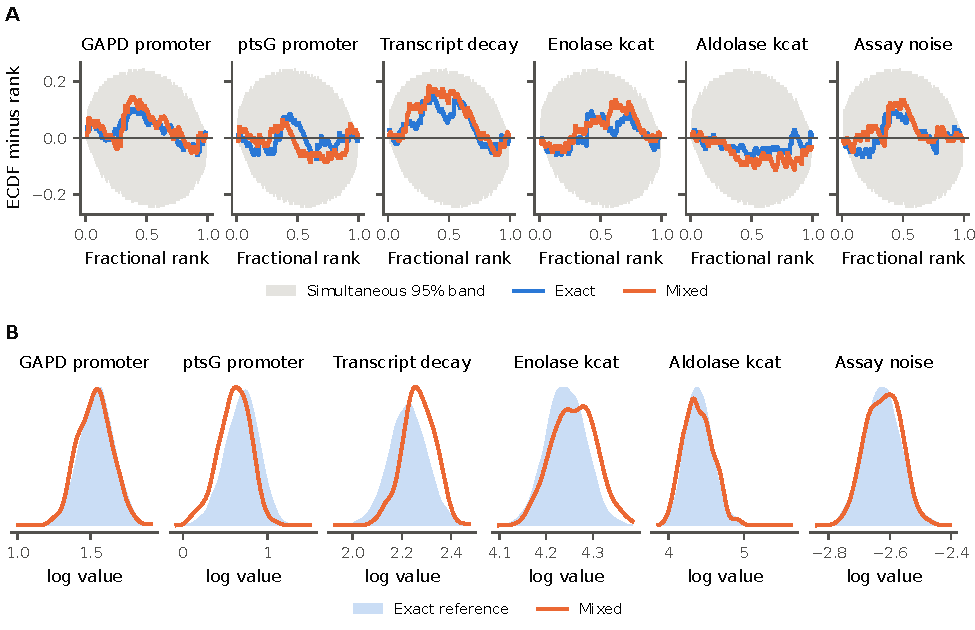
\includegraphics[width=\linewidth]{fig_mixed.pdf}
\caption{\textbf{Posteriors on M0, by both routes.} A: marginal posteriors of the natural log of each parameter on the reference dataset: the exact reference as a filled blue density, and the mixed route as the orange line. The ptsG promoter, the decay rate and enolase sit \pn{mix.gaplo}--\pn{mix.gaphi} standard deviations apart, and the cause is open. B: rank-ECDFs of both routes
over the same \pn{mix.R} prior-drawn datasets, against simultaneous bands at a joint level of 95\%. The grey region is the band, and each line is the rank-ECDF minus the fractional rank.}
\label{fig:approx}
\end{figure*}

\paragraph{The posteriors.} \Cref{fig:approx}A shows both routes on one M0 dataset of
\pn{mzero.cells} cells. The exact reference is \pn{vsix.chains} chains of \pn{vsix.sweeps} sweeps. Its rank-normalised $\Rhat$
\cite{vehtari2021rank} is at most \pn{vsix.rhat}, and its bulk effective sample
size is at least \pn{vsix.ess} for every parameter. The mixed route, which depends on a bulk covariance $S$ computed once from a hybrid ensemble (\cref{sec:meanfield}), uses
\pn{mix.chains} chains of \pn{mix.nadapt} adaptation and \pn{mix.ndraw}
sampling steps per dataset. On this dataset the ptsG promoter, the decay rate and
enolase sit \pn{mix.gaplo}--\pn{mix.gaphi} standard deviations from the exact
reference, about \pn{mix.gapfloor} above the matched noise floor, the largest distance between chains run under identical settings. Re-estimating $S$ at
the posterior mean does not close this gap, and its cause is open.

\paragraph{Are they calibrated?} A test against one known truth, as in DREAM8
\cite{karr2015summary}, cannot show whether a posterior's width is right. So we drew
\pn{vseven.R} parameter sets from the prior,
simulated one dataset from each, and fitted each dataset by each route, with one chain for the exact route. For each
parameter we compared the empirical CDF of the ranks of the truth with a
simultaneous band \cite{sailynoja2022graphical}, at a joint level of 95\% over the
\pn{mzero.npar} parameters. On both routes all \pn{mzero.npar} parameters stay inside their bands (\cref{fig:approx}B), a test that detects only large miscalibration at this size. A sampler that returned the prior would also pass, so we note that the exact reference does contract: on its dataset the posterior variance is about \pn{vsix.shrinklo}--\pn{vsix.shrinkhi}\% below the prior's. The largest deviation is \pn{vseven.maxdev} on the exact route and \pn{mix.sbcmax} on the mixed route, both for the
transcript decay rate, where the band allows \pn{vseven.band}. A calibration test
over many datasets does not exclude a gap of the size above on one dataset, so we report
both. \Cref{app:posteriors} gives the coverage read from the exact ranks.

\paragraph{What they cost.} A mixed posterior costs a median of \pn{mix.cpuh} CPU-hours
(range \pn{mix.cpuhlo}--\pn{mix.cpuhhi}), against \pn{ften.cpuh}--\pn{cost.exacthi}
for the exact sampler (\cref{tab:cost}). That median counts completed jobs only: a fault in the
starting optimiser lost another \pn{mix.lost} CPU-hours across the whole run. The long reference run cost
\pn{vsix.cpuh} CPU-hours. A production-length exact chain, about one-\pn{ften.speedup}th of that, is not distinguishable from the reference on
any marginal (\cref{app:posteriors}). An exact posterior on
the full reduced model is projected at about \pn{cost.fullscale} CPU-hours, above
our bound of \pn{cost.kone} CPU-hours per posterior. Exact inference therefore
stops at M0. The mixed route costs far less on M0, but we have not calibrated it on the
reduced model. The cost is the number of simulations, not the time of one. One cycle
of the full reduced model takes \pn{model.cyclewall}\,s, and a fast
implementation of the full \syn{} model is the subject of a companion paper
\cite{kimpson2026whole}.

\begin{table}[t]
\caption{\textbf{CPU-hours per posterior.} The mixed route's value is a median over completed jobs.}
\label{tab:cost}
\centering
\small
\begin{tabular}{@{}lcc@{}}
\toprule
Route & M0 & Reduced model \\
\midrule
Exact, reference & \pn{vsix.cpuh} & --- \\
Exact, production & \pn{ften.cpuh}--\pn{cost.exacthi} & $\sim$\pn{cost.fullscale} (projected) \\
Mixed & \pn{mix.cpuh} & not run \\
\bottomrule
\end{tabular}
\end{table}

\paragraph{How closely the routes agree.} Over the \pn{mix.R} datasets,
the largest mean bias of the mixed route against the exact posteriors is \pn{mix.biasmax}~$\pm$~\pn{mix.biasse} posterior standard deviations, for the decay rate. The median ratio of standard deviations per parameter is between \pn{mix.sdlo} and \pn{mix.sdhi}, and per parameter \pn{mix.mcselo}--\pn{mix.mcsehi} of the datasets differ from the exact fit by more than three of its Monte Carlo standard errors.

\paragraph{Limits.} The calibration results hold for M0 only. In \pn{vseven.lowess}
of the \pn{vseven.R} exact replicates the smallest bulk effective sample size is below 100, and autocorrelated draws can distort ranks. In \pn{mix.lowconv} of the \pn{mix.R} mixed replicates the two chains
fall short of $\Rhat \le 1.02$ and a bulk effective sample size of 100. The worst
$\Rhat$ is \pn{mix.rhat} and the smallest effective sample size is \pn{mix.ess}. The
mixed calibration result is unchanged without those replicates, as a sensitivity check only, since dropping them is a selection.


\stub{pointer: M0 detail in \cref{app:supporting}, holding $S$ fixed in \cref{app:sfixed}, the crossed comparison in \cref{app:crossed}.}
